\documentclass[10pt]{beamer}

\usetheme{Madrid}
\usecolortheme{default}
\setbeamertemplate{navigation symbols}{}
\setbeamersize{text margin left=0.6cm,text margin right=0.6cm}

\usepackage{tikz}
\usetikzlibrary{automata, positioning, arrows.meta, shapes.geometric, calc}
\usepackage{amsmath, amssymb}
\pdfstringdefDisableCommands{\def\translate#1{#1}}
\setbeamercovered{transparent=18}

\title{Properties of Regular Languages}
\subtitle{Closure, Decision Algorithms, and the Pumping Lemma}
\author{Computer Science Theory}
\date{Slide Set 4}

\begin{document}

\begin{frame}
  \titlepage
\end{frame}

\begin{frame}{Table of Contents}
  \tableofcontents
\end{frame}

\begin{frame}{Learning Outcomes}
  By the end of this slide set, you should be able to:
  \begin{itemize}
    \item prove closure of the regular languages using automaton
      constructions and set identities;
    \item decide membership, emptiness, finiteness, equality, containment, and
      universality for regular languages;
    \item state and explain the quantifier structure of the pumping lemma;
    \item use the pumping lemma to prove selected languages nonregular; and
    \item recognize invalid pumping-lemma arguments and repair them.
  \end{itemize}
\end{frame}

% ==========================================
% Part 1: Closure Properties
% ==========================================
\section{Closure Properties}

\begin{frame}{Part 1: Core Closure Properties}
  \textbf{Self-Study Header:} Operating within the Regular World
  \vspace{0.2cm}
  
  A class of languages is \textbf{closed} under an operation if applying that operation to members of the class always results in a member of the same class.
  \pause
  
  \begin{block}{Closure Theorem}
    The family of regular languages is closed under union, intersection,
    concatenation, complement, and Kleene star.
  \end{block}
  \pause
  
  Formally, if $L_1$ and $L_2$ are regular languages, the following are also regular:
  \begin{enumerate}
      \item \textbf{Union:} $L_1 \cup L_2$
      \item \textbf{Concatenation:} $L_1 L_2$
      \item \textbf{Kleene star:} $L_1^*$
      \item \textbf{Complement:} $\overline{L_1} = \Sigma^* \setminus L_1$
      \item \textbf{Intersection:} $L_1 \cap L_2$
  \end{enumerate}
\end{frame}

\begin{frame}{Proof by Construction: Union Using Grammars}
  \small
  \textbf{Theorem:} If $L_1$ and $L_2$ are regular, then
  $L_1\cup L_2$ is regular.
  \pause

  \begin{block}{Regular-Grammar Construction}
    Let $G_1=(V_1,\Sigma,S_1,P_1)$ and
    $G_2=(V_2,\Sigma,S_2,P_2)$ be right-linear grammars for $L_1$ and $L_2$.
    Rename variables so that $V_1\cap V_2=\varnothing$, and introduce a fresh
    start variable $S$.

    If unit productions are allowed, define
    \[
      G=(V_1\cup V_2\cup\{S\},\Sigma, S,
      P_1\cup P_2\cup\{S\to S_1\mid S_2\}).
    \]
  \end{block}
  \pause
  
  \begin{block}{Correctness}
    Every derivation begins by choosing $S\to S_1$ or $S\to S_2$ and then follows productions from the selected grammar. Therefore $L(G)=L(G_1)\cup L(G_2)=L_1\cup L_2$.

    %If unit productions are not permitted, replace $S\to S_i$ by copies of every production whose left-hand side is $S_i$. The resulting grammar is still right-linear and generates the same union.
  \end{block}
\end{frame}

\begin{frame}{Proof by Construction: Complementation}
  \textbf{Theorem:} If $L$ is regular, then $\overline{L}$ is regular.
  \pause
  \vspace{0.2cm}
  
  \begin{block}{The Construction}
    Because $L$ is regular, a \emph{complete} DFA
    $M=(Q,\Sigma,\delta,q_0,F)$ recognizes $L$.
    Construct $M'=(Q,\Sigma,\delta,q_0,Q\setminus F)$ by swapping the
    accepting and nonaccepting states.
  \end{block}
  \pause
  
  \begin{center}
  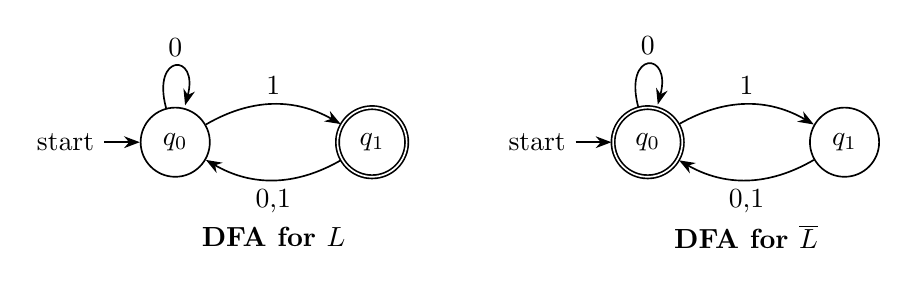
\begin{tikzpicture}[->, >=Stealth, auto, node distance=2.5cm, semithick]
    % Original DFA
    \node[state, initial] (q0) {$q_0$};
    \node[state, accepting] (q1) [right of=q0] {$q_1$};
    \path (q0) edge [bend left] node {1} (q1)
          (q0) edge [loop above] node {0} (q0)
          (q1) edge [bend left] node {0,1} (q0);
    \node at (1.25, -1.2) {\textbf{DFA for $L$}};
    
    % Complemented DFA
    \begin{scope}[xshift=6cm]
    \node[state, initial, accepting] (q0s) {$q_0$};
    \node[state] (q1s) [right of=q0s] {$q_1$};
    \path (q0s) edge [bend left] node {1} (q1s)
          (q0s) edge [loop above] node {0} (q0s)
          (q1s) edge [bend left] node {0,1} (q0s);
    \node at (1.25, -1.2) {\textbf{DFA for $\overline{L}$}};
    \end{scope}
  \end{tikzpicture}
  \end{center}
  \pause
  \textit{Crucial detail:} Complete the DFA first by adding a sink state if
  necessary. Merely swapping final states in an NFA does not compute the
  complement, because acceptance is existential over its possible paths.
\end{frame}

\begin{frame}{Proof by Construction: Intersection}
  \textbf{Theorem:} If $L_1$ and $L_2$ are regular, then $L_1 \cap L_2$ is regular.
  \pause
  
  \begin{block}{Cartesian Product Construction}
    Let $M_1=(Q_1,\Sigma,\delta_1,s_1,F_1)$ and
    $M_2=(Q_2,\Sigma,\delta_2,s_2,F_2)$.
    We build a new DFA $M_{\cap} = (Q, \Sigma, \delta, q_0, F)$ that simulates both machines simultaneously:
    \begin{itemize}
        \item $Q = Q_1 \times Q_2$ (the states are pairs).
        \item $\delta((r_1, r_2), a) = (\delta_1(r_1, a), \delta_2(r_2, a))$.
        \item $q_0 = (s_1, s_2)$.
        \item $F = F_1 \times F_2$ (accept iff \textbf{both} machines accept).
    \end{itemize}
  \end{block}
  \pause
  \begin{alertblock}{Alternative Proof via De Morgan's Law}
    Alternatively, $L_1 \cap L_2 = \overline{\overline{L_1} \cup \overline{L_2}}$. Since regular languages are closed under union and complementation, they must be closed under intersection!
  \end{alertblock}
\end{frame}

\begin{frame}{Advanced Operations}
  \small
  Regular languages are robust and closed under many other operations.
  \pause
  \begin{itemize}
      \item \textbf{Reversal ($L^R$):} Reverse every transition, make the old
        start state the sole accept state, and add a new start state with
        $\varepsilon$-transitions to all old accept states.
      \pause
      \item \textbf{Difference ($L_1 \setminus L_2$):} Since $L_1 \setminus L_2 = L_1 \cap \overline{L_2}$, and regular languages are closed under intersection and complement, they are closed under difference.
      \pause
      \item \textbf{Homomorphism ($h(L)$):} For each transition labeled $a$,
        replace the edge by a path spelling $h(a)$; use an
        $\varepsilon$-transition when $h(a)=\varepsilon$.
      \pause
      \item \textbf{Right quotient:}
        $L_1/L_2=\{x:\text{some }y\in L_2\text{ satisfies }xy\in L_1\}$.
        If $L_1$ and $L_2$ are regular, then $L_1/L_2$ is regular.
  \end{itemize}
\end{frame}

\begin{frame}{Closure Proof Toolbox}
  \small
  Choose the representation that makes the operation easiest.
  \begin{block}{Automaton Constructions}
    \begin{description}
      \item[Union/intersection:] Use a product DFA; change only the accepting
        pairs ($\lor$ for union, $\land$ for intersection).
      \item[Complement:] Complete a DFA and replace $F$ by $Q\setminus F$.
      \item[Concatenation/star:] Connect $\varepsilon$-NFAs using the same
        wrappers as in Thompson's construction.
      \item[Reversal:] Reverse the transitions and exchange the roles of the
        initial and final boundaries.
      \item[Homomorphism:] Replace each symbol edge by a path spelling its
        image.
    \end{description}
  \end{block}
  \pause
  \begin{exampleblock}{Set Identities Save Work}
    Difference, symmetric difference, and De Morgan's laws reduce new closure
    questions to operations already known to preserve regularity.
  \end{exampleblock}
\end{frame}

% ==========================================
% Part 2: Decision Algorithms
% ==========================================
\section{Decision Algorithms}

\begin{frame}{Part 2: Elementary Questions}
  \small
  \textbf{Self-Study Header:} Algorithmic Decidability
  \vspace{0.2cm}
  
  Given a standard representation of a regular language $L$ (DFA, NFA,
  regular expression, or regular grammar), can we algorithmically answer
  fundamental questions about it?
  \pause
  
  \begin{block}{1. The Membership Question}
    Given a string $w$ and a standard representation of $L$, is $w \in L$?
    \par\smallskip
    \textbf{Algorithm:} For a DFA, trace the unique path labeled $w$ from
    $q_0$ and test whether it ends in $F$.

    \textbf{Running time:} $O(|w|)$ for a supplied DFA. Converting an NFA, RE,
    or grammar to a DFA is preprocessing and may increase the representation
    size substantially.
  \end{block}
  \pause
  Because the standard representations are effectively convertible, a DFA
  algorithm establishes decidability for all of them, though not necessarily
  with the same complexity.
\end{frame}

\begin{frame}{Emptiness and Finiteness}
  \small
  \begin{block}{2. The Emptiness Question}
    Given a regular language $L$, is $L = \emptyset$?
    \par\smallskip
    \textbf{Algorithm:} Run BFS or DFS from $q_0$. The language is nonempty
    exactly when some state in $F$ is reachable.
  \end{block}
  \pause
  
  \begin{block}{3. The Finiteness Question}
    Given a regular language $L$, is $L$ finite or infinite?
    \par\smallskip
    \textbf{Algorithm:} Keep the \emph{useful} states that are reachable from
    $q_0$ and can reach a final state. Then $L$ is infinite exactly when the
    subgraph induced by these useful states contains a directed cycle.
  \end{block}
\end{frame}

\begin{frame}{The Equality Algorithm}
  \textbf{Question:} Given two regular languages $L_1$ and $L_2$, is $L_1 = L_2$?
  \pause
  
  We answer this using the \textbf{symmetric difference}:
  \[
    L_3=(L_1\cap\overline{L_2})\cup(\overline{L_1}\cap L_2).
  \]
  $L_3$ contains all strings that are in one language but not the other. $L_1 = L_2$ if and only if $L_3 = \emptyset$.
  \pause
  
  \begin{center}
  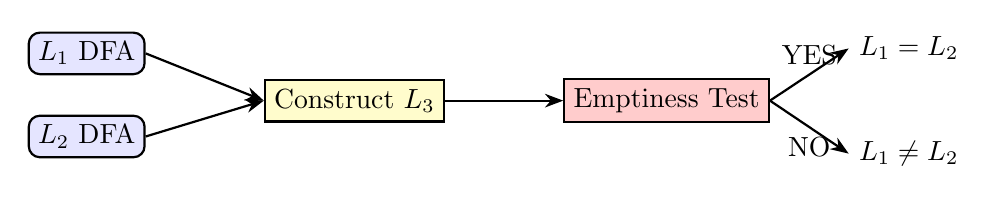
\begin{tikzpicture}[>=Stealth, node distance=1.5cm, auto, thick]
    \node[draw, rectangle, rounded corners, fill=blue!10] (L1) {$L_1$ DFA};
    \node[draw, rectangle, rounded corners, fill=blue!10] (L2) [below=0.5cm of L1] {$L_2$ DFA};
    
    \node[draw, rectangle, fill=yellow!20] (sym) [right=1.5cm of L1, yshift=-0.6cm] {Construct $L_3$};
    \node[draw, rectangle, fill=red!20] (empty) [right=1.5cm of sym] {Emptiness Test};
    
    \node (yes) [above right=0.1cm and 1cm of empty] {$L_1 = L_2$};
    \node (no) [below right=0.1cm and 1cm of empty] {$L_1 \neq L_2$};

    \draw[->] (L1.east) -- (sym.west);
    \draw[->] (L2.east) -- (sym.west);
    \draw[->] (sym.east) -- (empty.west);
    \draw[->] (empty.east) -- node[above] {YES} (yes.west);
    \draw[->] (empty.east) -- node[below] {NO} (no.west);
  \end{tikzpicture}
  \end{center}
\end{frame}

\begin{frame}{More Decidable Questions}
  \small
  Once emptiness and the product construction are available, several other
  questions follow immediately.
  \begin{block}{Reductions to Emptiness}
    \begin{align*}
      L=\Sigma^*
      &\Longleftrightarrow \overline{L}=\emptyset
      &&\text{(universality)},\\
      L_1\subseteq L_2
      &\Longleftrightarrow L_1\cap\overline{L_2}=\emptyset
      &&\text{(containment)},\\
      L_1\cap L_2=\emptyset
      &&&\text{(disjointness)}.
    \end{align*}
  \end{block}
  \pause
  \begin{exampleblock}{Direct Product Test}
    For equality, build the product DFA and search for a reachable pair in
    which exactly one component is accepting. Such a path labels a concrete
    counterexample string distinguishing the two languages.
  \end{exampleblock}
\end{frame}

% ==========================================
% Part 3: The Pumping Lemma
% ==========================================
\section{The Pumping Lemma}

\begin{frame}{Part 3: Concept \& The Pigeonhole Principle}
  \small
  \textbf{Self-Study Header:} The Limits of Finite Memory
  \vspace{0.2cm}
  
  A DFA has finite memory: its current state records everything relevant about
  the prefix read so far. What happens when a computation is longer than the
  number of available states?
  \pause
  
  \begin{block}{The Pigeonhole Principle}
    If $p$ pigeons are placed into fewer than $p$ holes, some hole has to have more than one pigeon in it. 
  \end{block}
  \pause
  If a DFA with $n$ states reads a string of length at least $n$, consider the
  states visited before reading any symbol and after each of the first $n$
  symbols. Among these $n+1$ visits, some state repeats. The intervening
  nonempty input labels a loop within the first $n$ symbols.
  
  \begin{center}
  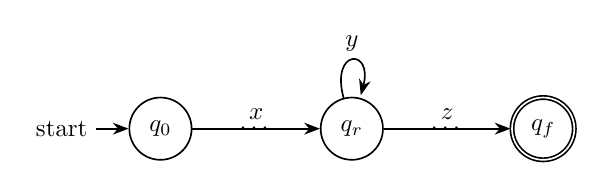
\begin{tikzpicture}[->, >=Stealth, auto, node distance=1.35cm, semithick,
      scale=0.9, transform shape]
    \node[state, initial] (q0) {$q_0$};
    \node (dots) [right of=q0] {$\dots$};
    \node[state] (qi) [right of=dots] {$q_r$};
    \node (dots2) [right of=qi] {$\dots$};
    \node[state, accepting] (qf) [right of=dots2] {$q_f$};
    
    \path (qi) edge [loop above] node {$y$} (qi)
          (q0) edge node {$x$} (qi)
          (qi) edge node {$z$} (qf);
  \end{tikzpicture}
  \end{center}
\end{frame}

\begin{frame}{Formal Statement: The Pumping Lemma}
  \small
  \begin{block}{Pumping lemma for regular languages}
    If $L$ is regular, then there exists $p\geq1$ such that every
    $s\in L$ with $|s|\geq p$ can be written as $s=xyz$ satisfying:
    \begin{enumerate}
        \item $xy^{i}z \in L$ for every $i\geq0$,
        \item $|y| > 0$, and
        \item $|xy| \leq p$.
    \end{enumerate}
  \end{block}
  \pause
  \vspace{0.2cm}
  \textbf{Breaking it down:}
  \begin{itemize}
      \item Condition 1: The same decomposition works for \emph{every}
        pumping value $i\geq0$.
      \item Condition 2: The loop consumes at least one symbol, so pumping
        actually changes the string when $i\neq1$.
      \item Condition 3: The loop lies within the first $p$ symbols.
  \end{itemize}
\end{frame}

\begin{frame}{Why the Pumping Lemma Is True}
  \small
  Let a DFA for $L$ have $p$ states, and let $s\in L$ with $|s|\geq p$.
  During the first $p$ input symbols, record the $p+1$ visited states:
  \[
    q_0,q_1,\ldots,q_p.
  \]
  Two visits must be equal; choose $0\leq r<t\leq p$ with $q_r=q_t$.
  Split $s$ as follows:
  \[
    \underbrace{s_1\cdots s_r}_{x}
    \underbrace{s_{r+1}\cdots s_t}_{y}
    \underbrace{s_{t+1}\cdots s_{|s|}}_{z}.
  \]
  Then $|y|=t-r>0$ and $|xy|=t\leq p$. Because reading $y$ returns the DFA
  to the same state, the loop may be traversed any number of times; hence
  $xy^{i}z\in L$ for every $i\geq0$.
\end{frame}

\begin{frame}{Quantifiers and the Lemma's Limitation}
  \small
  The logical order is the heart of a correct nonregularity proof:
  \[
    \exists p\ \forall s\ \exists(x,y,z)\ \forall i\geq0.
  \]
  To contradict the lemma, reverse the game after assuming regularity:
  \[
    \forall p\ \exists s\ \forall(x,y,z)\ \exists i\geq0
    \quad\text{such that }xy^{i}z\notin L,
  \]
  subject to $s=xyz$, $|s|\geq p$, $|y|>0$, and $|xy|\leq p$.
  \pause
  \begin{alertblock}{Necessary, Not Sufficient}
    Every regular language satisfies the pumping lemma, but satisfying the
    lemma does not by itself prove that a language is regular. Finite languages
    satisfy it vacuously by choosing $p$ larger than every string length.
  \end{alertblock}
\end{frame}

\begin{frame}{The Adversarial Game}
  The pumping lemma is used \textbf{negatively} to prove that a language is
  not regular. Its quantifiers can be remembered as a four-step game.
  \pause
  
  \begin{alertblock}{How to play the Pumping Game}
    \begin{enumerate}
        \item \textbf{Opponent:} Gives you the pumping length $p$ promised by
          the assumption that the language is regular.
        \pause
        \item \textbf{You:} Pick a strategic string $s \in L$ such that $|s| \geq p$.
        \pause
        \item \textbf{Opponent:} Chooses any valid split $s=xyz$ with
          $|y|>0$ and $|xy|\leq p$.
        \pause
        \item \textbf{You:} After seeing the split, choose $i\geq0$ so that
          $xy^{i}z\notin L$.
    \end{enumerate}
  \end{alertblock}
  \pause
  If this strategy works for every valid split, the initial regularity
  assumption is false.
\end{frame}

% ==========================================
% Part 4: Proving Non-Regularity
% ==========================================
\section{Proving Non-Regularity}

\begin{frame}{Example 1: Equal Blocks}
  \small
  \textbf{Goal:} Prove
  $L=\{a^n b^n:n\geq0\}$ is not regular.
  \pause
  
  \begin{enumerate}
      \item Assume $L$ is regular. The opponent provides pumping length $p$.
      \pause
      \item \textbf{We choose:} $s = a^p b^p$. Note that $s \in L$ and $|s| = 2p \geq p$.
      \pause
      \item Opponent divides $s=xyz$.

      \textit{Crucial insight:} Since $|xy|\leq p$, both $x$ and $y$ lie in
      the first block of $a$'s. Thus $y=a^k$ for some $1\leq k\leq p$.
      \pause
      \item \textbf{We pump:} Choose $i = 2$. The new string is $xy^2z$.
      \begin{itemize}
          \item $s = xy^1z$ had $p$ $a$'s and $p$ $b$'s.
          \item Pumping adds $k$ extra $a$'s.
          \item The new string $xy^2z = a^{p+k} b^p$.
      \end{itemize}
  \end{enumerate}
  \pause
  Since $k>0$, the numbers of $a$'s and $b$'s differ. Thus
  $xy^2z\notin L$, contradicting the pumping lemma. Therefore $L$ is not
  regular.
\end{frame}

\begin{frame}{Example 2: Duplicated Strings}
  \small
  \textbf{Goal:} Prove
  $F=\{ww:w\in\{0,1\}^{*}\}$ is not regular.
  \pause
  
  \begin{enumerate}
      \item Assume $F$ is regular. Opponent provides pumping length $p$.
      \pause
      \item \textbf{We choose:} $s=0^p10^p1=(0^p1)(0^p1)$.
      \pause
      \item Because $|xy|\leq p$, a valid split has $y=0^k$ for some
        $1\leq k\leq p$.
      \pause
      \item \textbf{We pump:} Choose $i = 2$. The new string is $xy^2z$.
      \begin{itemize}
          \item The first block of $0$'s now has $p+k$ zeros.
          \item The new string is $0^{p+k} 1 0^p 1$.
      \end{itemize}
  \end{enumerate}
  \pause
  The pumped string has exactly two $1$'s, separated by $p+1$ positions. If it
  were $uu$, the distance between these two corresponding $1$'s would equal
  half the total length, $p+1+k/2$, which is impossible for $k>0$ (and if $k$
  is odd, the total length is odd). Hence $xy^2z\notin F$, a contradiction.
\end{frame}

\begin{frame}{Example 3: Unary Perfect Squares}
  \small
  \textbf{Goal:} Prove
  $L=\{a^{n^2}:n\geq0\}$ is not regular.
  \pause
  
  \begin{center}
  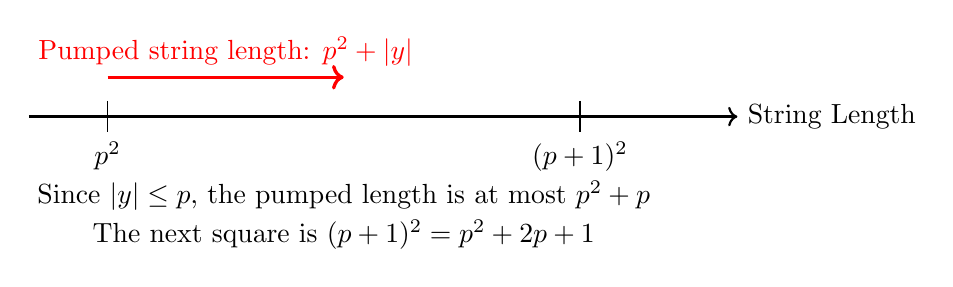
\begin{tikzpicture}
    % Number line
    \draw[thick, ->] (0,0) -- (9,0) node[right] {String Length};
    
    % Points
    \draw (1,0.2) -- (1,-0.2) node[below] {$p^2$};
    \draw (7,0.2) -- (7,-0.2) node[below] {$(p+1)^2$};
    
    % Pumped string
    \draw[->, red, very thick] (1, 0.5) -- (4, 0.5) node[midway, above] {Pumped string length: $p^2 + |y|$};
    
    % Explanation
    \node at (4, -1) {Since $|y|\leq p$, the pumped length is at most $p^2+p$};
    \node at (4, -1.5) {The next square is $(p+1)^2=p^2+2p+1$};
  \end{tikzpicture}
  \end{center}
  \pause
  
  \begin{enumerate}
      \item Pick $s = a^{p^2}$. Opponent divides $s = xyz$.
      \item We pump $i=2$. The length of $xy^2z$ is $p^2 + |y|$.
      \item Since $|y| \leq p$, then
        $p^2<p^2+|y|\leq p^2+p<p^2+2p+1=(p+1)^{2}$.
  \end{enumerate}
  \pause
  The pumped length lies strictly between consecutive squares, so
  $xy^2z\notin L$. This contradicts the pumping lemma.
\end{frame}

\begin{frame}{Using Closure to Prove Nonregularity}
  \small
  Closure theorems can be used contrapositively.
  \begin{block}{Reduction Pattern}
    To prove a language $K$ nonregular:
    \begin{enumerate}
      \item assume $K$ is regular;
      \item apply an operation that preserves regularity; and
      \item obtain a language already known to be nonregular.
    \end{enumerate}
  \end{block}
  \pause
  \begin{exampleblock}{Example}
    Let
    \[
      K=\{w\in\{a,b\}^{*}:|w|_a=|w|_b\}.
    \]
    If $K$ were regular, then its intersection with the regular language
    $a^{*}b^{*}$ would be regular. But
    \[
      K\cap a^{*}b^{*}=\{a^n b^n:n\geq0\},
    \]
    contradicting Example~1. Hence $K$ is not regular.
  \end{exampleblock}
\end{frame}

% ==========================================
% Pedagogical Enhancements
% ==========================================
\section{Review and Exercises}

\begin{frame}{Checkpoint Exercises}
  \small
  \begin{enumerate}
      \item \textbf{Closure Property Trap:} Given that $L_1$ is regular, and the union $L_1 \cup L_2$ is regular, does it necessarily follow that $L_2$ is regular?
      \pause
      \vspace{0.4cm}
      \item \textbf{A Surprising Result:} Let $D$ contain the strings over
        $\{0,1\}$ having equally many occurrences of $01$ and $10$ as
        consecutive substrings. Is $D$ regular?
      \pause
      \vspace{0.4cm}
      \item \textbf{Choosing $s$:} If trying to prove $L = \{a^n b^n \mid n \geq 0\}$ is not regular, what is wrong with picking $s = a^2 b^2$ if the opponent's $p=5$?
  \end{enumerate}
\end{frame}

\begin{frame}{Teacher's Corner: Common Pitfalls}
  \small
  \begin{alertblock}{Pitfall 1: Picking a specific $p$}
    Students sometimes begin by fixing $p=5$. This is invalid: the pumping
    length is an unknown constant. The strategy must work for every $p\geq1$.
  \end{alertblock}
  \pause
  \begin{alertblock}{Pitfall 2: Making assumptions about $y$}
    Even for $s=a^{p}b^{p}$, you may not assume $y=a$. The opponent may choose
    $y=a^k$ for any $1\leq k\leq p$. The proof succeeds because pumping
    \emph{every} such nonempty block changes only the number of $a$'s.

    Also verify $s\in L$: for example,
    $(ab)^{p}\notin\{a^{n}b^{n}:n\geq0\}$ when
    $p>1$, so it cannot be used as the witness string for Example~1.
  \end{alertblock}
\end{frame}

\begin{frame}{Hints for Checkpoint Exercises}
  \small
  \begin{block}{Hints and Solutions}
    \begin{itemize}
        \item \textbf{Exercise 1 (Closure Trap):} False. Let
        $L_1=\Sigma^*$. Then $L_1\cup L_2=\Sigma^*$ for any $L_2$, including
        a nonregular language.
        \vspace{0.3cm}
        \item \textbf{Exercise 2 (01 and 10 substrings):} Yes. Each change
        $0\to1$ must eventually be balanced by a change $1\to0$, except for a
        possible net change determined by the endpoints. Thus the counts are
        equal exactly for $\varepsilon$ or when the first and last symbols
        agree; a DFA need only remember the first and current symbols.
        \vspace{0.3cm}
        \item \textbf{Exercise 3 (Choosing $s$):} The witness must satisfy
        $|s|\geq p$. If $p=5$, then $|a^2b^2|=4$, so the pumping lemma makes
        no promise about that string.
    \end{itemize}
  \end{block}
  \pause
  \vspace{0.2cm}
  \textbf{Pro-Tip: Pumping Down}\par
  Sometimes pumping up ($i=2$) does not break the defining property. The
  lemma also requires $xy^0z=xz\in L$, so deleting $y$ is often the cleaner
  route to a contradiction.
\end{frame}

\appendix
\section{Appendix: Extended Problems and Theory}

\begin{frame}{Appendix Road Map}
  \small
  This appendix provides optional material for tutorials, examinations, and
  advanced self-study:
  \begin{enumerate}
    \item five additional pumping-lemma proofs in adversarial-game form;
    \item constructive proofs for homomorphism and right quotient;
    \item solved book-style challenges on regular-language properties; and
    \item advanced results: Myhill--Nerode, residual languages, Arden's lemma,
      inverse homomorphisms, and state complexity.
  \end{enumerate}
  \begin{block}{Suggested use}
    Select only the examples that match the class level. The main lecture is
    complete without the appendix.
  \end{block}
\end{frame}

% ==========================================
% Appendix A: More Pumping-Lemma Games
% ==========================================
\subsection{Additional Pumping-Lemma Games}

\begin{frame}{Pumping Game A: Binary Palindromes}
  \small
  Prove
  \[
    L=\{w\in\{0,1\}^*:w=w^R\}
  \]
  is not regular.
  \begin{alertblock}{Adversarial solution}
    \begin{enumerate}
      \item \textbf{Opponent:} Supplies pumping length $p$.
      \item \textbf{You:} Choose $s=0^p10^p$, a palindrome.
      \item \textbf{Opponent:} Chooses $s=xyz$ with
        $|xy|\le p$ and $|y|>0$. Hence $y=0^k$ for some $1\le k\le p$.
      \item \textbf{You:} Pump down with $i=0$:
        \[
          xz=0^{p-k}10^p.
        \]
    \end{enumerate}
  \end{alertblock}
  The two sides of the central $1$ now have different lengths, so $xz$ is not
  a palindrome. This contradicts the pumping lemma.
\end{frame}

\begin{frame}{Pumping Game B: Unary Prime Lengths}
  \small
  Let
  \[
    L=\{a^q:q\text{ is prime}\}.
  \]
  Assume $L$ is regular.
  \begin{alertblock}{Adversarial solution}
    \begin{enumerate}
      \item \textbf{Opponent:} Supplies pumping length $p$.
      \item \textbf{You:} Choose a prime $q\ge p$ and set $s=a^q$.
      \item \textbf{Opponent:} Chooses $s=xyz$. Since the alphabet is unary,
        $y=a^k$ for some $1\le k\le p$.
      \item \textbf{You:} Choose $i=q+1$. The pumped length is
        \[
          |xy^{q+1}z|=q+qk=q(k+1).
        \]
    \end{enumerate}
  \end{alertblock}
  Both factors exceed $1$, so the new length is composite. Therefore the
  pumped string is not in $L$, a contradiction.
\end{frame}

\begin{frame}{Pumping Game C: Powers of Two}
  \small
  Prove
  \[
    L=\{a^{2^n}:n\ge0\}
  \]
  is not regular.
  \begin{alertblock}{Adversarial solution}
    \begin{enumerate}
      \item \textbf{Opponent:} Supplies pumping length $p$.
      \item \textbf{You:} Choose $m$ so that $2^m>p$ and let $s=a^{2^m}$.
      \item \textbf{Opponent:} Chooses $s=xyz$, where
        $y=a^k$ and $1\le k\le p$.
      \item \textbf{You:} Pump up once, choosing $i=2$. The new length is
        $2^m+k$.
    \end{enumerate}
  \end{alertblock}
  Because
  \[
    2^m<2^m+k<2^m+2^m=2^{m+1},
  \]
  the pumped length lies strictly between consecutive powers of two.
\end{frame}

\begin{frame}{Pumping Game D: More Zeros Than Ones}
  \small
  Let
  \[
    L=\{0^n1^m:n>m\ge0\}.
  \]
  Assume $L$ is regular.
  \begin{alertblock}{Adversarial solution}
    \begin{enumerate}
      \item \textbf{Opponent:} Supplies pumping length $p$.
      \item \textbf{You:} Choose $s=0^p1^{p-1}\in L$.
      \item \textbf{Opponent:} Chooses $s=xyz$ with $|xy|\le p$; therefore
        $y=0^k$ for some $1\le k\le p$.
      \item \textbf{You:} Pump down:
        \[
          xz=0^{p-k}1^{p-1}.
        \]
    \end{enumerate}
  \end{alertblock}
  Since $p-k\le p-1$, the number of zeros is no longer strictly greater than
  the number of ones. Thus $xz\notin L$.
\end{frame}

\begin{frame}{Pumping Game E: A Divisibility Constraint}
  \small
  Prove that
  \[
    L=\{a^n b^m:n,m\ge1\text{ and }n\mid m\}
  \]
  is not regular.
  \begin{alertblock}{Adversarial solution}
    \begin{enumerate}
      \item \textbf{Opponent:} Supplies pumping length $p$.
      \item \textbf{You:} Choose $s=a^pb^p\in L$ because $p\mid p$.
      \item \textbf{Opponent:} Chooses $s=xyz$. The prefix restriction forces
        $y=a^k$ for some $1\le k\le p$.
      \item \textbf{You:} Pump with $i=2$, obtaining
        \[
          xy^2z=a^{p+k}b^p.
        \]
    \end{enumerate}
  \end{alertblock}
  A positive integer $p+k>p$ cannot divide the smaller positive integer $p$.
  Hence the pumped string is not in $L$.
\end{frame}

% ==========================================
% Appendix B: Homomorphism and Quotient
% ==========================================
\subsection{Homomorphism and Right Quotient}

\begin{frame}{Homomorphisms: Definition and Closure Theorem}
  \small
  A homomorphism $h:\Sigma^*\to\Gamma^*$ is determined by its values on
  symbols and extended by
  \[
    h(\varepsilon)=\varepsilon,
    \qquad
    h(a_1\cdots a_n)=h(a_1)\cdots h(a_n).
  \]
  \begin{block}{Theorem}
    If $L$ is regular, then its homomorphic image
    $h(L)=\{h(w):w\in L\}$ is regular.
  \end{block}
  \begin{block}{Automaton construction}
    Let an automaton $M$ recognize $L$. For every transition
    $q\xrightarrow{a}r$:
    \begin{itemize}
      \item replace it by a path spelling $h(a)$, using fresh intermediate
        states when $|h(a)|>1$;
      \item use an $\varepsilon$-transition when $h(a)=\varepsilon$.
    \end{itemize}
    Keep the original start and accepting states. The result is an
    $\varepsilon$-NFA.
  \end{block}
  A path labeled $w$ in $M$ becomes a path labeled $h(w)$ in the new
  automaton, proving that its language is exactly $h(L)$.
\end{frame}

\begin{frame}{Worked Homomorphism Examples}
  \footnotesize
  Let $L=(01)^*$.
  \begin{exampleblock}{Non-erasing homomorphism}
    If $h(0)=ab$ and $h(1)=c$, then
    \[
      h(L)=\{(abc)^n:n\ge0\}=(abc)^*.
    \]
    Every transition on $0$ is replaced by a two-edge path labeled $a,b$,
    and every transition on $1$ becomes a $c$-edge.
  \end{exampleblock}
  \begin{exampleblock}{Erasing homomorphism}
    If $g(0)=ab$ and $g(1)=\varepsilon$, then
    \[
      g(L)=(ab)^*.
    \]
    The $1$-transition becomes an $\varepsilon$-move.
  \end{exampleblock}
  \begin{alertblock}{Common distinction}
    Homomorphic images may merge distinct source words or erase symbols.
    Closure states that the resulting language remains regular; it does not
    claim that $h$ is one-to-one.
  \end{alertblock}
\end{frame}

\begin{frame}{Right Quotient: Constructive Closure Proof}
  \small
  The right quotient of $L_1$ by $L_2$ is
  \[
    L_1/L_2=\{x:\text{there exists }y\in L_2\text{ with }xy\in L_1\}.
  \]
  \begin{block}{Theorem}
    If $L_1$ and $L_2$ are regular, then $L_1/L_2$ is regular.
  \end{block}
  Let $M_1=(Q,\Sigma,\delta,q_0,F)$ recognize $L_1$. Define
  \[
    F'=\{q\in Q:\exists y\in L_2,\ \delta^*(q,y)\in F\}.
  \]
  Use the DFA
  \[
    M'=(Q,\Sigma,\delta,q_0,F').
  \]
  After reading $x$, $M'$ accepts precisely when some suffix $y\in L_2$
  can take the current state to an old accepting state. Therefore
  \[
    x\in L(M')\iff\exists y\in L_2:xy\in L_1.
  \]
  The set $F'$ is computable by product-graph reachability using DFAs for
  $L_1$ and $L_2$.
\end{frame}

\begin{frame}{Worked Right-Quotient Examples}
  \footnotesize
  \begin{exampleblock}{Removing one required suffix}
    Let $L_1=(ab)^*$ and $L_2=\{b\}$. Then
    \[
      L_1/L_2
      =\{x:xb\in(ab)^*\}
      =(ab)^*a.
    \]
    For example, $aba\in L_1/L_2$ because $abab\in(ab)^*$.
  \end{exampleblock}
  \begin{exampleblock}{A family of possible suffixes}
    Over $\Sigma=\{0,1\}$, let
    $L_1=\Sigma^*01$ and $L_2=1^*$. Then
    \[
      L_1/L_2=\Sigma^*0\ \cup\ \Sigma^*01.
    \]
    The empty suffix keeps every word already ending in $01$; a nonempty
    suffix from $1^*$ can complete any word ending in $0$.
  \end{exampleblock}
  \begin{alertblock}{Advanced remark}
    For a fixed regular $L_1$, $L_1/L_2$ is regular even for arbitrary
    $L_2$, because only a subset of the finitely many states becomes final.
    Regularity of $L_2$ makes that subset effectively computable.
  \end{alertblock}
\end{frame}

% ==========================================
% Appendix C: Solved Book-Style Challenges
% ==========================================
\subsection{Solved Book-Style Challenges}

\begin{frame}{Challenge 1: Prefixes, Suffixes, and Factors}
  \small
  For a language $L$, define
  \[
    \begin{aligned}
      \operatorname{Pref}(L)&=\{x:\exists y,\ xy\in L\},\\
      \operatorname{Suff}(L)&=\{y:\exists x,\ xy\in L\},\\
      \operatorname{Fact}(L)&=\{z:\exists x,y,\ xzy\in L\}.
    \end{aligned}
  \]
  \begin{block}{Claim}
    If $L$ is regular, all three languages are regular.
  \end{block}
  \textbf{Solution.}
  Let $M$ be a DFA for $L$.
  \begin{itemize}
    \item For prefixes, make accepting every state that can reach an old
      accepting state.
    \item For suffixes, use an NFA whose possible start states are all states
      reachable from the original start.
    \item For factors, combine both changes: start at any reachable state and
      accept at any state that can reach an old final state.
  \end{itemize}
  Each construction has finitely many states, proving regularity.
\end{frame}

\begin{frame}{Challenge 2: Infinite Regular Subsets}
  \small
  \begin{block}{Problem}
    Prove that every infinite regular language contains an infinite regular
    sublanguage.
  \end{block}
  \textbf{Solution.}
  Let $p$ be a pumping length for an infinite regular language $L$.
  Choose $s\in L$ with $|s|\ge p$, and take the decomposition
  $s=xyz$ guaranteed by the pumping lemma. Then
  \[
    R=\{xy^iz:i\ge0\}
  \]
  is a subset of $L$. Since $|y|>0$, these strings have distinct lengths, so
  $R$ is infinite. Moreover,
  \[
    R=\{x\}\{y\}^*\{z\},
  \]
  which is regular by closure under concatenation and star.
  \begin{exampleblock}{Lesson}
    An infinite regular language always contains an explicitly describable
    ultimately periodic family.
  \end{exampleblock}
\end{frame}

\begin{frame}{Challenge 3: A Short Witness of Infinitude}
  \small
  \begin{block}{Problem}
    Let a DFA have $n$ states. Prove that its language is infinite iff it
    accepts some word $w$ satisfying
    \[
      n\le |w|<2n.
    \]
  \end{block}
  \textbf{Forward direction.}
  Choose a shortest accepted word of length at least $n$. If its length were
  at least $2n$, a repeated state among the first $n+1$ visits would identify
  a loop of length at most $n$. Removing that loop would leave an accepted
  word still of length at least $n$, contradicting minimality.

  \textbf{Reverse direction.}
  Any accepted word of length at least $n$ repeats a state along its path.
  Pumping the resulting nonempty loop yields infinitely many accepted words.
  \begin{block}{Algorithmic consequence}
    Finiteness can be tested by searching useful cycles, or equivalently by
    testing acceptance at lengths $n,\ldots,2n-1$.
  \end{block}
\end{frame}

\begin{frame}{Challenge 4: How Long Is a Counterexample?}
  \small
  \begin{block}{Problem}
    DFA $M_1$ has $m$ states and DFA $M_2$ has $n$ states. If their languages
    differ, show that some distinguishing string has length less than $mn$.
  \end{block}
  \textbf{Solution.}
  Build the product DFA for the symmetric difference. It has at most $mn$
  states and accepts exactly the strings on which the two machines disagree.
  If the languages differ, an accepting product state is reachable.

  Choose a shortest path to such a state. It cannot repeat a product state;
  otherwise deleting the intervening cycle would give a shorter accepting
  path. A simple path through at most $mn$ states has at most $mn-1$ edges.
  Therefore a distinguishing string exists with
  \[
    |w|\le mn-1.
  \]
  \begin{exampleblock}{Practical use}
    Breadth-first search in the product not only decides equivalence but
    returns a shortest counterexample.
  \end{exampleblock}
\end{frame}

\begin{frame}{Challenge 5: Counting $01$ and $10$}
  \small
  Let $N_{01}(w)$ and $N_{10}(w)$ count overlapping adjacent occurrences.
  Determine whether
  \[
    D=\{w:N_{01}(w)=N_{10}(w)\}
  \]
  is regular.
  \begin{block}{Key invariant}
    For every nonempty binary string,
    \[
      N_{01}(w)-N_{10}(w)=
      \begin{cases}
        1,&w\text{ starts with }0\text{ and ends with }1,\\
       -1,&w\text{ starts with }1\text{ and ends with }0,\\
        0,&w\text{ has equal first and last symbols}.
      \end{cases}
    \]
  \end{block}
  Each change from $0$ to $1$ is canceled by a later change back, except for
  the net change between the endpoints. Hence
  \[
    D=\{\varepsilon\}\cup\{0,1\}
      \cup0\Sigma^*0\cup1\Sigma^*1,
  \]
  which is regular. A DFA need only remember the first and current symbols.
\end{frame}

\begin{frame}{About the Book-Style Challenges}
  \small
  The preceding problems are newly phrased solutions based on recurring
  exercise themes in standard theory-of-computation texts:
  \begin{itemize}
    \item closure constructions and decision algorithms;
    \item pumping consequences for infinite regular languages;
    \item product automata and shortest distinguishing strings; and
    \item finding a finite invariant for a seemingly unbounded counting
      property.
  \end{itemize}
  \begin{alertblock}{Study method}
    Before reading a solution, identify the most useful representation:
    DFA graph, product automaton, regular expression, closure identity, or
    pumping loop. The representation usually reveals the proof.
  \end{alertblock}
\end{frame}

% ------------------------------------------
% Advanced structural results
% ------------------------------------------
\subsection{Advanced Theorems and Observations}

\begin{frame}{Myhill--Nerode: The Exact Regularity Test}
  \small
  For a language $L\subseteq\Sigma^*$, define
  \[
    x\equiv_L y
    \quad\Longleftrightarrow\quad
    \text{for every }z\in\Sigma^*,\;
    xz\in L\Longleftrightarrow yz\in L.
  \]
  Thus $x$ and $y$ are equivalent when no future suffix can distinguish
  them.
  \pause
  \begin{block}{Myhill--Nerode Theorem}
    $L$ is regular if and only if $\equiv_L$ has finitely many equivalence
    classes. Moreover, the number of classes equals the number of states in
    the minimal DFA for $L$.
  \end{block}
  \pause
  \begin{exampleblock}{Interpretation}
    A DFA state represents all prefixes having the same possible futures.
    Minimization merges exactly the states whose prefixes cannot be
    distinguished by any continuation.
  \end{exampleblock}
\end{frame}

\begin{frame}{Myhill--Nerode Nonregularity Proof}
  \small
  Prove again that
  \[
    L=\{a^n b^n:n\ge0\}
  \]
  is not regular.
  \pause
  Consider the infinite collection of prefixes
  $\varepsilon,a,a^2,a^3,\ldots$. If $i<j$, choose the distinguishing suffix
  $z=b^i$. Then
  \[
    a^i z=a^i b^i\in L,
    \qquad
    a^j z=a^j b^i\notin L.
  \]
  Therefore $a^i\not\equiv_L a^j$ whenever $i\ne j$.
  \pause

  The relation $\equiv_L$ has infinitely many classes, so the
  Myhill--Nerode theorem implies that $L$ is not regular.
  \begin{alertblock}{Compared with pumping}
    The pumping lemma gives a necessary property of regular languages.
    Myhill--Nerode gives an exact characterization and also explains the
    state count of the minimal DFA.
  \end{alertblock}
\end{frame}

\begin{frame}{Residual Languages and the Minimal DFA}
  \small
  The \textbf{left quotient} or \textbf{residual} of $L$ by a word $x$ is
  \[
    x^{-1}L=\{z\in\Sigma^*:xz\in L\}.
  \]
  It records all suffixes that can complete the prefix $x$ into a word of
  $L$.
  \pause
  \begin{block}{Structural facts}
    \begin{itemize}
      \item $x\equiv_L y$ exactly when $x^{-1}L=y^{-1}L$.
      \item The distinct residuals of a regular language can serve as the
        states of its minimal DFA.
      \item The start state is $\varepsilon^{-1}L=L$; a residual is accepting
        exactly when it contains $\varepsilon$.
      \item Reading $a$ moves $x^{-1}L$ to $(xa)^{-1}L$.
    \end{itemize}
  \end{block}
  Hence the minimal DFA is unique up to renaming states: its states are the
  language's intrinsically different future behaviors.
\end{frame}

\begin{frame}{Arden's Lemma: Solving Language Equations}
  \small
  \begin{block}{Arden's Lemma}
    If $X,A,B\subseteq\Sigma^*$ satisfy
    \[
      X=AX\cup B
    \]
    and $\varepsilon\notin A$, then the unique solution is
    \[
      X=A^*B.
    \]
  \end{block}
  \pause
  Indeed, repeatedly substituting for $X$ gives
  $X=B\cup AB\cup A^2B\cup\cdots=A^*B$. The condition
  $\varepsilon\notin A$ guarantees uniqueness.
  \pause
  \begin{exampleblock}{Example}
    The equation $X=aX\cup b$ has solution
    \[
      X=a^*b.
    \]
    Systems of such equations provide a systematic route from a finite
    automaton to a regular expression.
  \end{exampleblock}
\end{frame}

\begin{frame}{Inverse Homomorphisms Preserve Regularity}
  \small
  For a homomorphism $h:\Sigma^*\to\Gamma^*$ and
  $L\subseteq\Gamma^*$, define
  \[
    h^{-1}(L)=\{w\in\Sigma^*:h(w)\in L\}.
  \]
  \pause
  Let $M=(Q,\Gamma,\delta,q_0,F)$ be a DFA for $L$. Construct a DFA over
  $\Sigma$ with the same states, start state, and final states, but define
  \[
    \delta'(q,a)=\delta^*(q,h(a)).
  \]
  By induction on $w$,
  $\delta'^*(q_0,w)=\delta^*(q_0,h(w))$. Thus the new DFA accepts $w$
  exactly when $h(w)\in L$.
  \pause
  \begin{exampleblock}{Example}
    If $h(0)=ab$, $h(1)=a$, and $L=(ab)^*$, then
    $h^{-1}(L)=0^*$: every $0$ contributes one $ab$, while any $1$ leaves an
    unmatched $a$.
  \end{exampleblock}
\end{frame}

\begin{frame}{State Complexity: Construction Size Matters}
  \small
  Closure proves that a result is regular; \textbf{state complexity} asks how
  large a recognizing DFA may need to be.
  \pause
  \begin{center}
  \begin{tabular}{l l}
    \textbf{Operation or conversion} & \textbf{General upper bound}\\
    \hline
    complement of an $n$-state complete DFA & $n$ states\\
    union/intersection of $m$- and $n$-state DFAs & $mn$ states\\
    determinization of an $n$-state NFA & $2^n$ subset states\\
    reversal of an $n$-state DFA & at most $2^n$ DFA states
  \end{tabular}
  \end{center}
  \pause
  These are worst-case bounds: unreachable or equivalent constructed states
  may be removed, although suitable language families attain exponential or
  product-size growth.
  \begin{alertblock}{Practical lesson}
    A mathematically simple closure construction can cause a substantial
    representation blow-up. Build reachable states on demand and minimize
    only when the application benefits from it.
  \end{alertblock}
\end{frame}

\begin{frame}{Further Regular-Language Observations}
  \small
  \begin{itemize}
    \item Every finite language is regular, and every infinite regular
      language contains an infinite regular sublanguage.
    \pause
    \item A unary regular language has an \emph{ultimately periodic} set of
      accepted lengths: after some point, membership repeats with a fixed
      period.
    \pause
    \item Two DFA states are inequivalent exactly when some suffix is accepted
      from one state and rejected from the other; partition refinement finds
      these equivalence classes efficiently.
    \pause
    \item The pumping length may be chosen as the number of states of a DFA,
      but it need not be the smallest possible pumping length for the
      language.
    \pause
    \item Regular expressions, right-linear grammars, DFAs, and NFAs have the
      same expressive power, but conversions between them can change the
      representation size dramatically.
  \end{itemize}
\end{frame}

\begin{frame}{Appendix References and Further Practice}
  \footnotesize
  \begin{thebibliography}{9}
    \bibitem{linz}
      Peter Linz and Susan H. Rodger,
      \newblock \emph{An Introduction to Formal Languages and Automata}, 7th ed.,
      \newblock Jones \& Bartlett Learning, 2023.

    \bibitem{sipser}
      Michael Sipser,
      \newblock \emph{Introduction to the Theory of Computation}, 3rd ed.,
      \newblock Cengage Learning, 2013.

    \bibitem{hopcroft}
      John E. Hopcroft, Rajeev Motwani, and Jeffrey D. Ullman,
      \newblock \emph{Introduction to Automata Theory, Languages, and
      Computation}, 3rd ed.,
      \newblock Pearson, 2006.
  \end{thebibliography}
  The appendix problems are original formulations of standard exercise
  themes; consult these texts for further variations on closure, minimization,
  language equations, and nonregularity proofs.
\end{frame}

\end{document}
